\documentclass[a4paper]{article}
\usepackage[]{graphicx}\usepackage[]{color}
% maxwidth is the original width if it is less than linewidth
% otherwise use linewidth (to make sure the graphics do not exceed the margin)
\makeatletter
\def\maxwidth{ %
  \ifdim\Gin@nat@width>\linewidth
    \linewidth
  \else
    \Gin@nat@width
  \fi
}
\makeatother

\definecolor{fgcolor}{rgb}{0.345, 0.345, 0.345}
\newcommand{\hlnum}[1]{\textcolor[rgb]{0.686,0.059,0.569}{#1}}%
\newcommand{\hlstr}[1]{\textcolor[rgb]{0.192,0.494,0.8}{#1}}%
\newcommand{\hlcom}[1]{\textcolor[rgb]{0.678,0.584,0.686}{\textit{#1}}}%
\newcommand{\hlopt}[1]{\textcolor[rgb]{0,0,0}{#1}}%
\newcommand{\hlstd}[1]{\textcolor[rgb]{0.345,0.345,0.345}{#1}}%
\newcommand{\hlkwa}[1]{\textcolor[rgb]{0.161,0.373,0.58}{\textbf{#1}}}%
\newcommand{\hlkwb}[1]{\textcolor[rgb]{0.69,0.353,0.396}{#1}}%
\newcommand{\hlkwc}[1]{\textcolor[rgb]{0.333,0.667,0.333}{#1}}%
\newcommand{\hlkwd}[1]{\textcolor[rgb]{0.737,0.353,0.396}{\textbf{#1}}}%
\let\hlipl\hlkwb

\usepackage{framed}
\makeatletter
\newenvironment{kframe}{%
 \def\at@end@of@kframe{}%
 \ifinner\ifhmode%
  \def\at@end@of@kframe{\end{minipage}}%
  \begin{minipage}{\columnwidth}%
 \fi\fi%
 \def\FrameCommand##1{\hskip\@totalleftmargin \hskip-\fboxsep
 \colorbox{shadecolor}{##1}\hskip-\fboxsep
     % There is no \\@totalrightmargin, so:
     \hskip-\linewidth \hskip-\@totalleftmargin \hskip\columnwidth}%
 \MakeFramed {\advance\hsize-\width
   \@totalleftmargin\z@ \linewidth\hsize
   \@setminipage}}%
 {\par\unskip\endMakeFramed%
 \at@end@of@kframe}
\makeatother

\definecolor{shadecolor}{rgb}{.97, .97, .97}
\definecolor{messagecolor}{rgb}{0, 0, 0}
\definecolor{warningcolor}{rgb}{1, 0, 1}
\definecolor{errorcolor}{rgb}{1, 0, 0}
\newenvironment{knitrout}{}{} % an empty environment to be redefined in TeX

\usepackage{alltt}
\newcommand{\SweaveOpts}[1]{}  % do not interfere with LaTeX
\newcommand{\SweaveInput}[1]{} % because they are not real TeX commands
\newcommand{\Sexpr}[1]{}       % will only be parsed by R



\usepackage[utf8]{inputenc}
\pagenumbering{arabic}
%\usepackage[ngerman]{babel}
\usepackage{a4wide,paralist}
\usepackage{amsmath, amssymb, xfrac, amsthm}
\usepackage{dsfont}
\usepackage[usenames,dvipsnames]{xcolor}
\usepackage{amsfonts}
\usepackage{graphicx}
\usepackage{caption}
\usepackage{subcaption}
\usepackage{framed}
\usepackage{multirow}
\usepackage{bytefield}
\usepackage{csquotes}
\usepackage[breakable, theorems, skins]{tcolorbox}
\usepackage{hyperref}
\usepackage{cancel}
\usepackage{bm}

\usepackage{bbm}
% basic latex stuff
\newcommand{\pkg}[1]{{\fontseries{b}\selectfont #1}} %fontstyle for R packages
\newcommand{\lz}{\vspace{0.5cm}} %vertical space
\newcommand{\dlz}{\vspace{1cm}} %double vertical space
\newcommand{\oneliner}[1] % Oneliner for important statements
{\begin{block}{}\begin{center}\begin{Large}#1\end{Large}\end{center}\end{block}}


%new environments
\newenvironment{vbframe}  %frame with breaks and verbatim
{
 \begin{frame}[containsverbatim,allowframebreaks]
}
{
\end{frame}
}

\newenvironment{vframe}  %frame with verbatim without breaks (to avoid numbering one slided frames)
{
 \begin{frame}[containsverbatim]
}
{
\end{frame}
}

\newenvironment{blocki}[1]   % itemize block
{
 \begin{block}{#1}\begin{itemize}
}
{
\end{itemize}\end{block}
}

\newenvironment{fragileframe}[2]{  %fragile frame with framebreaks
\begin{frame}[allowframebreaks, fragile, environment = fragileframe]
\frametitle{#1}
#2}
{\end{frame}}


\newcommand{\myframe}[2]{  %short for frame with framebreaks
\begin{frame}[allowframebreaks]
\frametitle{#1}
#2
\end{frame}}

\newcommand{\remark}[1]{
  \textbf{Remark:} #1
}

\newcommand{\citebutton}[2]{%
\NoCaseChange{\resizebox{!}{9pt}{\protect\beamergotobutton{\href{#2}{#1}}}}%
}



\newenvironment{deleteframe}
{
\begingroup
\usebackgroundtemplate{\includegraphics[width=\paperwidth,height=\paperheight]{../style/color/red.png}}
 \begin{frame}
}
{
\end{frame}
\endgroup
}
\newenvironment{simplifyframe}
{
\begingroup
\usebackgroundtemplate{\includegraphics[width=\paperwidth,height=\paperheight]{../style/color/yellow.png}}
 \begin{frame}
}
{
\end{frame}
\endgroup
}\newenvironment{draftframe}
{
\begingroup
\usebackgroundtemplate{\includegraphics[width=\paperwidth,height=\paperheight]{../style/color/green.jpg}}
 \begin{frame}
}
{
\end{frame}
\endgroup
}
% https://tex.stackexchange.com/a/261480: textcolor that works in mathmode
\makeatletter
\renewcommand*{\@textcolor}[3]{%
  \protect\leavevmode
  \begingroup
    \color#1{#2}#3%
  \endgroup
}
\makeatother


\tcbset{enhanced}

%exercise numbering
\renewcommand{\theenumi}{(\alph{enumi})}
\renewcommand{\theenumii}{\roman{enumii}}
\renewcommand\labelenumi{\theenumi}

\font \sfbold=cmssbx10
\setlength{\oddsidemargin}{0cm} \setlength{\textwidth}{16cm}

\sloppy
\parindent0em
\parskip0.5em
\topmargin-2.3 cm
\textheight25cm
\textwidth17.5cm
\oddsidemargin-0.8cm
% \pagestyle{empty}

\newcommand{\kopf}[1] {
\hrule
\vspace{.15cm}
\begin{minipage}{\textwidth}
	{\sf \bf \huge Exercise Collection -- #1}
\end{minipage}
\vspace{.05cm}
\hrule
\vspace{1cm}}

\newcommand{\exlect}
  {\color{black} \hrule \section{Lecture exercises}}
  
\newcommand{\exexams}
  {\color{black} \hrule \section{Questions from past exams}}
  
\newcommand{\exinspo}
  {\color{black} \hrule \section{Ideas \& exercises from other sources}}

\newcounter{aufg}
\newenvironment{aufgabe}[1]
	{\color{black} \refstepcounter{aufg}
	\subsection{Exercise \arabic{aufg}: #1} 
	\noindent}
	{\vspace{0.5cm}}
	
\newenvironment{aufgabeexam}[3] % semester, main or retry exam, question number
	{\color{black} \refstepcounter{aufg}
	\subsection{Exercise \arabic{aufg}: #1, #2 exam, question #3}
	\noindent}
	{\vspace{1.5cm}}

\newcounter{loes}
\newenvironment{loesung}
	{\color{gray} \refstepcounter{loes}\textbf{Solution \arabic{loes}:}
	\\ \noindent}
	{\bigskip}

\setcounter{secnumdepth}{0}



\begin{document}
% !Rnw weave = knitr



% math spaces
\ifdefined\N                                                                
\renewcommand{\N}{\mathds{N}} % N, naturals
\else \newcommand{\N}{\mathds{N}} \fi 
\newcommand{\Z}{\mathds{Z}} % Z, integers
\newcommand{\Q}{\mathds{Q}} % Q, rationals
\newcommand{\R}{\mathds{R}} % R, reals
\ifdefined\C 
  \renewcommand{\C}{\mathds{C}} % C, complex
\else \newcommand{\C}{\mathds{C}} \fi
\newcommand{\continuous}{\mathcal{C}} % C, space of continuous functions
\newcommand{\M}{\mathcal{M}} % machine numbers
\newcommand{\epsm}{\epsilon_m} % maximum error

% counting / finite sets
\newcommand{\setzo}{\{0, 1\}} % set 0, 1
\newcommand{\setmp}{\{-1, +1\}} % set -1, 1
\newcommand{\unitint}{[0, 1]} % unit interval

% basic math stuff
\newcommand{\xt}{\tilde x} % x tilde
\newcommand{\argmax}{\operatorname{arg\,max}} % argmax
\newcommand{\argmin}{\operatorname{arg\,min}} % argmin
\newcommand{\argminlim}{\mathop{\mathrm{arg\,min}}\limits} % argmax with limits
\newcommand{\argmaxlim}{\mathop{\mathrm{arg\,max}}\limits} % argmin with limits  
\newcommand{\sign}{\operatorname{sign}} % sign, signum
\newcommand{\I}{\mathbb{I}} % I, indicator
\newcommand{\order}{\mathcal{O}} % O, order
\newcommand{\pd}[2]{\frac{\partial{#1}}{\partial #2}} % partial derivative
\newcommand{\floorlr}[1]{\left\lfloor #1 \right\rfloor} % floor
\newcommand{\ceillr}[1]{\left\lceil #1 \right\rceil} % ceiling

% sums and products
\newcommand{\sumin}{\sum\limits_{i=1}^n} % summation from i=1 to n
\newcommand{\sumim}{\sum\limits_{i=1}^m} % summation from i=1 to m
\newcommand{\sumjn}{\sum\limits_{j=1}^n} % summation from j=1 to p
\newcommand{\sumjp}{\sum\limits_{j=1}^p} % summation from j=1 to p
\newcommand{\sumik}{\sum\limits_{i=1}^k} % summation from i=1 to k
\newcommand{\sumkg}{\sum\limits_{k=1}^g} % summation from k=1 to g
\newcommand{\sumjg}{\sum\limits_{j=1}^g} % summation from j=1 to g
\newcommand{\meanin}{\frac{1}{n} \sum\limits_{i=1}^n} % mean from i=1 to n
\newcommand{\meanim}{\frac{1}{m} \sum\limits_{i=1}^m} % mean from i=1 to n
\newcommand{\meankg}{\frac{1}{g} \sum\limits_{k=1}^g} % mean from k=1 to g
\newcommand{\prodin}{\prod\limits_{i=1}^n} % product from i=1 to n
\newcommand{\prodkg}{\prod\limits_{k=1}^g} % product from k=1 to g
\newcommand{\prodjp}{\prod\limits_{j=1}^p} % product from j=1 to p

% linear algebra
\newcommand{\one}{\boldsymbol{1}} % 1, unitvector
\newcommand{\zero}{\mathbf{0}} % 0-vector
\newcommand{\id}{\boldsymbol{I}} % I, identity
\newcommand{\diag}{\operatorname{diag}} % diag, diagonal
\newcommand{\trace}{\operatorname{tr}} % tr, trace
\newcommand{\spn}{\operatorname{span}} % span
\newcommand{\scp}[2]{\left\langle #1, #2 \right\rangle} % <.,.>, scalarproduct
\newcommand{\mat}[1]{\begin{pmatrix} #1 \end{pmatrix}} % short pmatrix command
\newcommand{\Amat}{\mathbf{A}} % matrix A
\newcommand{\Deltab}{\mathbf{\Delta}} % error term for vectors

% basic probability + stats
\renewcommand{\P}{\mathds{P}} % P, probability
\newcommand{\E}{\mathds{E}} % E, expectation
\newcommand{\var}{\mathsf{Var}} % Var, variance
\newcommand{\cov}{\mathsf{Cov}} % Cov, covariance
\newcommand{\corr}{\mathsf{Corr}} % Corr, correlation
\newcommand{\normal}{\mathcal{N}} % N of the normal distribution
\newcommand{\iid}{\overset{i.i.d}{\sim}} % dist with i.i.d superscript
\newcommand{\distas}[1]{\overset{#1}{\sim}} % ... is distributed as ...

% machine learning
\newcommand{\Xspace}{\mathcal{X}} % X, input space
\newcommand{\Yspace}{\mathcal{Y}} % Y, output space
\newcommand{\nset}{\{1, \ldots, n\}} % set from 1 to n
\newcommand{\pset}{\{1, \ldots, p\}} % set from 1 to p
\newcommand{\gset}{\{1, \ldots, g\}} % set from 1 to g
\newcommand{\Pxy}{\mathbb{P}_{xy}} % P_xy
\newcommand{\Exy}{\mathbb{E}_{xy}} % E_xy: Expectation over random variables xy
\newcommand{\xv}{\mathbf{x}} % vector x (bold)
\newcommand{\xtil}{\tilde{\mathbf{x}}} % vector x-tilde (bold)
\newcommand{\yv}{\mathbf{y}} % vector y (bold)
\newcommand{\xy}{(\xv, y)} % observation (x, y)
\newcommand{\xvec}{\left(x_1, \ldots, x_p\right)^\top} % (x1, ..., xp) 
\newcommand{\Xmat}{\mathbf{X}} % Design matrix
\newcommand{\allDatasets}{\mathds{D}} % The set of all datasets
\newcommand{\allDatasetsn}{\mathds{D}_n}  % The set of all datasets of size n 
\newcommand{\D}{\mathcal{D}} % D, data
\newcommand{\Dn}{\D_n} % D_n, data of size n
\newcommand{\Dtrain}{\mathcal{D}_{\text{train}}} % D_train, training set
\newcommand{\Dtest}{\mathcal{D}_{\text{test}}} % D_test, test set
\newcommand{\xyi}[1][i]{\left(\xv^{(#1)}, y^{(#1)}\right)} % (x^i, y^i), i-th observation
\newcommand{\Dset}{\left( \xyi[1], \ldots, \xyi[n]\right)} % {(x1,y1)), ..., (xn,yn)}, data
\newcommand{\defAllDatasetsn}{(\Xspace \times \Yspace)^n} % Def. of the set of all datasets of size n 
\newcommand{\defAllDatasets}{\bigcup_{n \in \N}(\Xspace \times \Yspace)^n} % Def. of the set of all datasets 
\newcommand{\xdat}{\left\{ \xv^{(1)}, \ldots, \xv^{(n)}\right\}} % {x1, ..., xn}, input data
\newcommand{\yvec}{\left(y^{(1)}, \hdots, y^{(n)}\right)^\top} % (y1, ..., yn), vector of outcomes
\renewcommand{\xi}[1][i]{\xv^{(#1)}} % x^i, i-th observed value of x
\newcommand{\yi}[1][i]{y^{(#1)}} % y^i, i-th observed value of y 
\newcommand{\xivec}{\left(x^{(i)}_1, \ldots, x^{(i)}_p\right)^\top} % (x1^i, ..., xp^i), i-th observation vector
\newcommand{\xj}{\xv_j} % x_j, j-th feature
\newcommand{\xjvec}{\left(x^{(1)}_j, \ldots, x^{(n)}_j\right)^\top} % (x^1_j, ..., x^n_j), j-th feature vector
\newcommand{\phiv}{\mathbf{\phi}} % Basis transformation function phi
\newcommand{\phixi}{\mathbf{\phi}^{(i)}} % Basis transformation of xi: phi^i := phi(xi)

%%%%%% ml - models general
\newcommand{\lamv}{\bm{\lambda}} % lambda vector, hyperconfiguration vector
\newcommand{\Lam}{\bm{\Lambda}}	 % Lambda, space of all hpos
% Inducer / Inducing algorithm
\newcommand{\preimageInducer}{\left(\defAllDatasets\right)\times\Lam} % Set of all datasets times the hyperparameter space
\newcommand{\preimageInducerShort}{\allDatasets\times\Lam} % Set of all datasets times the hyperparameter space
% Inducer / Inducing algorithm
\newcommand{\ind}{\mathcal{I}} % Inducer, inducing algorithm, learning algorithm 

% continuous prediction function f
\newcommand{\ftrue}{f_{\text{true}}}  % True underlying function (if a statistical model is assumed)
\newcommand{\ftruex}{\ftrue(\xv)} % True underlying function (if a statistical model is assumed)
\newcommand{\fx}{f(\xv)} % f(x), continuous prediction function
\newcommand{\fdomains}{f: \Xspace \rightarrow \R^g} % f with domain and co-domain
\newcommand{\Hspace}{\mathcal{H}} % hypothesis space where f is from
\newcommand{\fbayes}{f^{\ast}} % Bayes-optimal model
\newcommand{\fxbayes}{f^{\ast}(\xv)} % Bayes-optimal model
\newcommand{\fkx}[1][k]{f_{#1}(\xv)} % f_j(x), discriminant component function
\newcommand{\fh}{\hat{f}} % f hat, estimated prediction function
\newcommand{\fxh}{\fh(\xv)} % fhat(x)
\newcommand{\fxt}{f(\xv ~|~ \thetab)} % f(x | theta)
\newcommand{\fxi}{f\left(\xv^{(i)}\right)} % f(x^(i))
\newcommand{\fxih}{\hat{f}\left(\xv^{(i)}\right)} % f(x^(i))
\newcommand{\fxit}{f\left(\xv^{(i)} ~|~ \thetab\right)} % f(x^(i) | theta)
\newcommand{\fhD}{\fh_{\D}} % fhat_D, estimate of f based on D
\newcommand{\fhDtrain}{\fh_{\Dtrain}} % fhat_Dtrain, estimate of f based on D
\newcommand{\fhDnlam}{\fh_{\Dn, \lamv}} %model learned on Dn with hp lambda
\newcommand{\fhDlam}{\fh_{\D, \lamv}} %model learned on D with hp lambda
\newcommand{\fhDnlams}{\fh_{\Dn, \lamv^\ast}} %model learned on Dn with optimal hp lambda 
\newcommand{\fhDlams}{\fh_{\D, \lamv^\ast}} %model learned on D with optimal hp lambda 

% discrete prediction function h
\newcommand{\hx}{h(\xv)} % h(x), discrete prediction function
\newcommand{\hh}{\hat{h}} % h hat
\newcommand{\hxh}{\hat{h}(\xv)} % hhat(x)
\newcommand{\hxt}{h(\xv | \thetab)} % h(x | theta)
\newcommand{\hxi}{h\left(\xi\right)} % h(x^(i))
\newcommand{\hxit}{h\left(\xi ~|~ \thetab\right)} % h(x^(i) | theta)
\newcommand{\hbayes}{h^{\ast}} % Bayes-optimal classification model
\newcommand{\hxbayes}{h^{\ast}(\xv)} % Bayes-optimal classification model

% yhat
\newcommand{\yh}{\hat{y}} % yhat for prediction of target
\newcommand{\yih}{\hat{y}^{(i)}} % yhat^(i) for prediction of ith targiet
\newcommand{\resi}{\yi- \yih}

% theta
\newcommand{\thetah}{\hat{\theta}} % theta hat
\newcommand{\thetab}{\bm{\theta}} % theta vector
\newcommand{\thetabh}{\bm{\hat\theta}} % theta vector hat
\newcommand{\thetat}[1][t]{\thetab^{[#1]}} % theta^[t] in optimization
\newcommand{\thetatn}[1][t]{\thetab^{[#1 +1]}} % theta^[t+1] in optimization
\newcommand{\thetahDnlam}{\thetabh_{\Dn, \lamv}} %theta learned on Dn with hp lambda
\newcommand{\thetahDlam}{\thetabh_{\D, \lamv}} %theta learned on D with hp lambda
\newcommand{\mint}{\min_{\thetab \in \Theta}} % min problem theta
\newcommand{\argmint}{\argmin_{\thetab \in \Theta}} % argmin theta

% densities + probabilities
% pdf of x 
\newcommand{\pdf}{p} % p
\newcommand{\pdfx}{p(\xv)} % p(x)
\newcommand{\pixt}{\pi(\xv~|~ \thetab)} % pi(x|theta), pdf of x given theta
\newcommand{\pixit}{\pi\left(\xi ~|~ \thetab\right)} % pi(x^i|theta), pdf of x given theta
\newcommand{\pixii}{\pi\left(\xi\right)} % pi(x^i), pdf of i-th x 

% pdf of (x, y)
\newcommand{\pdfxy}{p(\xv,y)} % p(x, y)
\newcommand{\pdfxyt}{p(\xv, y ~|~ \thetab)} % p(x, y | theta)
\newcommand{\pdfxyit}{p\left(\xi, \yi ~|~ \thetab\right)} % p(x^(i), y^(i) | theta)

% pdf of x given y
\newcommand{\pdfxyk}[1][k]{p(\xv | y= #1)} % p(x | y = k)
\newcommand{\lpdfxyk}[1][k]{\log p(\xv | y= #1)} % log p(x | y = k)
\newcommand{\pdfxiyk}[1][k]{p\left(\xi | y= #1 \right)} % p(x^i | y = k)

% prior probabilities
\newcommand{\pik}[1][k]{\pi_{#1}} % pi_k, prior
\newcommand{\lpik}[1][k]{\log \pi_{#1}} % log pi_k, log of the prior
\newcommand{\pit}{\pi(\thetab)} % Prior probability of parameter theta

% posterior probabilities
\newcommand{\post}{\P(y = 1 ~|~ \xv)} % P(y = 1 | x), post. prob for y=1
\newcommand{\postk}[1][k]{\P(y = #1 ~|~ \xv)} % P(y = k | y), post. prob for y=k
\newcommand{\pidomains}{\pi: \Xspace \rightarrow \unitint} % pi with domain and co-domain
\newcommand{\pibayes}{\pi^{\ast}} % Bayes-optimal classification model
\newcommand{\pixbayes}{\pi^{\ast}(\xv)} % Bayes-optimal classification model
\newcommand{\pix}{\pi(\xv)} % pi(x), P(y = 1 | x)
\newcommand{\pikx}[1][k]{\pi_{#1}(\xv)} % pi_k(x), P(y = k | x)
\newcommand{\pikxt}[1][k]{\pi_{#1}(\xv ~|~ \thetab)} % pi_k(x | theta), P(y = k | x, theta)
\newcommand{\pixh}{\hat \pi(\xv)} % pi(x) hat, P(y = 1 | x) hat
\newcommand{\pikxh}[1][k]{\hat \pi_{#1}(\xv)} % pi_k(x) hat, P(y = k | x) hat
\newcommand{\pixih}{\hat \pi(\xi)} % pi(x^(i)) with hat
\newcommand{\pikxih}[1][k]{\hat \pi_{#1}(\xi)} % pi_k(x^(i)) with hat
\newcommand{\pdfygxt}{p(y ~|~\xv, \thetab)} % p(y | x, theta)
\newcommand{\pdfyigxit}{p\left(\yi ~|~\xi, \thetab\right)} % p(y^i |x^i, theta)
\newcommand{\lpdfygxt}{\log \pdfygxt } % log p(y | x, theta)
\newcommand{\lpdfyigxit}{\log \pdfyigxit} % log p(y^i |x^i, theta)

% probababilistic
\newcommand{\bayesrulek}[1][k]{\frac{\P(\xv | y= #1) \P(y= #1)}{\P(\xv)}} % Bayes rule
\newcommand{\muk}{\bm{\mu_k}} % mean vector of class-k Gaussian (discr analysis) 

% residual and margin
\newcommand{\eps}{\epsilon} % residual, stochastic
\newcommand{\epsi}{\epsilon^{(i)}} % epsilon^i, residual, stochastic
\newcommand{\epsh}{\hat{\epsilon}} % residual, estimated
\newcommand{\yf}{y \fx} % y f(x), margin
\newcommand{\yfi}{\yi \fxi} % y^i f(x^i), margin
\newcommand{\Sigmah}{\hat \Sigma} % estimated covariance matrix
\newcommand{\Sigmahj}{\hat \Sigma_j} % estimated covariance matrix for the j-th class

% ml - loss, risk, likelihood
\newcommand{\Lyf}{L\left(y, f\right)} % L(y, f), loss function
\newcommand{\Lxy}{L\left(y, \fx\right)} % L(y, f(x)), loss function
\newcommand{\Lxyi}{L\left(\yi, \fxi\right)} % loss of observation
\newcommand{\Lxyt}{L\left(y, \fxt\right)} % loss with f parameterized
\newcommand{\Lxyit}{L\left(\yi, \fxit\right)} % loss of observation with f parameterized
\newcommand{\Lxym}{L\left(\yi, f\left(\bm{\tilde{x}}^{(i)} ~|~ \thetab\right)\right)} % loss of observation with f parameterized
\newcommand{\Lpixy}{L\left(y, \pix\right)} % loss in classification
\newcommand{\Lpixyi}{L\left(\yi, \pixii\right)} % loss of observation in classification
\newcommand{\Lpixyt}{L\left(y, \pixt\right)} % loss with pi parameterized
\newcommand{\Lpixyit}{L\left(\yi, \pixit\right)} % loss of observation with pi parameterized
\newcommand{\Lhxy}{L\left(y, \hx\right)} % L(y, h(x)), loss function on discrete classes
\newcommand{\Lr}{L\left(r\right)} % L(r), loss defined on residual (reg) / margin (classif)
\newcommand{\lone}{|y - \fx|} % L1 loss
\newcommand{\ltwo}{\left(y - \fx\right)^2} % L2 loss
\newcommand{\lbernoullimp}{\ln(1 + \exp(-y \cdot \fx))} % Bernoulli loss for -1, +1 encoding
\newcommand{\lbernoullizo}{- y \cdot \fx + \log(1 + \exp(\fx))} % Bernoulli loss for 0, 1 encoding
\newcommand{\lcrossent}{- y \log \left(\pix\right) - (1 - y) \log \left(1 - \pix\right)} % cross-entropy loss
\newcommand{\lbrier}{\left(\pix - y \right)^2} % Brier score
\newcommand{\risk}{\mathcal{R}} % R, risk
\newcommand{\riskbayes}{\mathcal{R}^\ast}
\newcommand{\riskf}{\risk(f)} % R(f), risk
\newcommand{\riskdef}{\E_{y|\xv}\left(\Lxy \right)} % risk def (expected loss)
\newcommand{\riskt}{\mathcal{R}(\thetab)} % R(theta), risk
\newcommand{\riske}{\mathcal{R}_{\text{emp}}} % R_emp, empirical risk w/o factor 1 / n
\newcommand{\riskeb}{\bar{\mathcal{R}}_{\text{emp}}} % R_emp, empirical risk w/ factor 1 / n
\newcommand{\riskef}{\riske(f)} % R_emp(f)
\newcommand{\risket}{\mathcal{R}_{\text{emp}}(\thetab)} % R_emp(theta)
\newcommand{\riskr}{\mathcal{R}_{\text{reg}}} % R_reg, regularized risk
\newcommand{\riskrt}{\mathcal{R}_{\text{reg}}(\thetab)} % R_reg(theta)
\newcommand{\riskrf}{\riskr(f)} % R_reg(f)
\newcommand{\riskrth}{\hat{\mathcal{R}}_{\text{reg}}(\thetab)} % hat R_reg(theta)
\newcommand{\risketh}{\hat{\mathcal{R}}_{\text{emp}}(\thetab)} % hat R_emp(theta)
\newcommand{\LL}{\mathcal{L}} % L, likelihood
\newcommand{\LLt}{\mathcal{L}(\thetab)} % L(theta), likelihood
\newcommand{\LLtx}{\mathcal{L}(\thetab | \xv)} % L(theta|x), likelihood
\newcommand{\logl}{\ell} % l, log-likelihood
\newcommand{\loglt}{\logl(\thetab)} % l(theta), log-likelihood
\newcommand{\logltx}{\logl(\thetab | \xv)} % l(theta|x), log-likelihood
\newcommand{\errtrain}{\text{err}_{\text{train}}} % training error
\newcommand{\errtest}{\text{err}_{\text{test}}} % test error
\newcommand{\errexp}{\overline{\text{err}_{\text{test}}}} % avg training error

% lm
\newcommand{\thx}{\thetab^\top \xv} % linear model
\newcommand{\olsest}{(\Xmat^\top \Xmat)^{-1} \Xmat^\top \yv} % OLS estimator in LM 


\kopf{Random Forests}

\tableofcontents

% ------------------------------------------------------------------------------
% LECTURE EXERCISES
% ------------------------------------------------------------------------------

\dlz
\exlect
\lz

\aufgabe{random forests vs CART}{

Try to find or simulate (at least) one 2 dimensional classification dataset as an example in which random forests can separate both classes well but CART is problematic. Hint: Have a look at the \texttt{mlbench} package.
}

\dlz
\loesung{

Try to find or simulate (at least) one 2 dimensional classification dataset as an example in which random forests can separate both classes well but CART is problematic. Hint: Have a look at the \texttt{mlbench} package.

\begin{knitrout}
\definecolor{shadecolor}{rgb}{0.969, 0.969, 0.969}\color{fgcolor}\begin{kframe}
\begin{alltt}
\hlkwd{library}\hlstd{(mlr3)}
\hlkwd{library}\hlstd{(mlr3learners)}
\hlkwd{library}\hlstd{(mlr3viz)}
\hlkwd{library}\hlstd{(mlbench)}
\hlkwd{library}\hlstd{(ggplot2)}
\hlkwd{library}\hlstd{(gridExtra)}

\hlkwd{set.seed}\hlstd{(}\hlnum{123}\hlstd{)}

\hlcom{# create learners}

\hlstd{rp} \hlkwb{=} \hlstd{mlr3}\hlopt{::}\hlkwd{lrn}\hlstd{(}\hlstr{"classif.rpart"}\hlstd{)}
\hlstd{rf} \hlkwb{=} \hlstd{mlr3}\hlopt{::}\hlkwd{lrn}\hlstd{(}\hlstr{"classif.ranger"}\hlstd{)}

\hlcom{# create two example data and corresponding tasks for mlr3}

\hlstd{data.spirals} \hlkwb{=} \hlstd{data.table}\hlopt{::}\hlkwd{as.data.table}\hlstd{(}
  \hlkwd{mlbench.spirals}\hlstd{(}\hlkwc{n} \hlstd{=} \hlnum{1000}\hlstd{,} \hlkwc{cycles} \hlstd{=} \hlnum{3}\hlstd{,} \hlkwc{sd} \hlstd{=} \hlnum{0.05}\hlstd{))}
\hlstd{task.spirals} \hlkwb{=} \hlstd{mlr3}\hlopt{::}\hlstd{TaskClassif}\hlopt{$}\hlkwd{new}\hlstd{(}
  \hlstr{"spirals"}\hlstd{,}
  \hlkwc{backend} \hlstd{= data.spirals,}
  \hlkwc{target} \hlstd{=} \hlstr{"classes"}\hlstd{)}
\hlstd{data.circle} \hlkwb{=} \hlstd{data.table}\hlopt{::}\hlkwd{as.data.table}\hlstd{(}\hlkwd{mlbench.circle}\hlstd{(}\hlnum{1000}\hlstd{,} \hlkwc{d} \hlstd{=} \hlnum{2}\hlstd{))}
\hlstd{task.circle} \hlkwb{=} \hlstd{mlr3}\hlopt{::}\hlstd{TaskClassif}\hlopt{$}\hlkwd{new}\hlstd{(}
  \hlstr{"circle"}\hlstd{,}
  \hlkwc{backend} \hlstd{= data.circle,}
  \hlkwc{target} \hlstd{=} \hlstr{"classes"}\hlstd{)}

\hlcom{# show how learners perform}

\hlstd{spirals1} \hlkwb{=} \hlstd{mlr3viz}\hlopt{::}\hlkwd{plot_learner_prediction}\hlstd{(rp, task.spirals)} \hlopt{+}
  \hlkwd{guides}\hlstd{(}\hlkwc{shape} \hlstd{=} \hlnum{FALSE}\hlstd{)}
\end{alltt}
\begin{verbatim}
## INFO  [17:12:22.739] [mlr3]  Applying learner 'classif.rpart' on task 'spirals' (iter 1/1)
\end{verbatim}
\begin{alltt}
\hlstd{spirals2} \hlkwb{=} \hlstd{mlr3viz}\hlopt{::}\hlkwd{plot_learner_prediction}\hlstd{(rf, task.spirals)} \hlopt{+}
  \hlkwd{guides}\hlstd{(}\hlkwc{shape} \hlstd{=} \hlnum{FALSE}\hlstd{)}
\end{alltt}
\begin{verbatim}
## INFO  [17:12:23.080] [mlr3]  Applying learner 'classif.ranger' on task 'spirals' (iter 1/1)
\end{verbatim}
\begin{alltt}
\hlkwd{grid.arrange}\hlstd{(spirals1, spirals2,} \hlkwc{ncol} \hlstd{=} \hlnum{2}\hlstd{)}
\end{alltt}
\end{kframe}
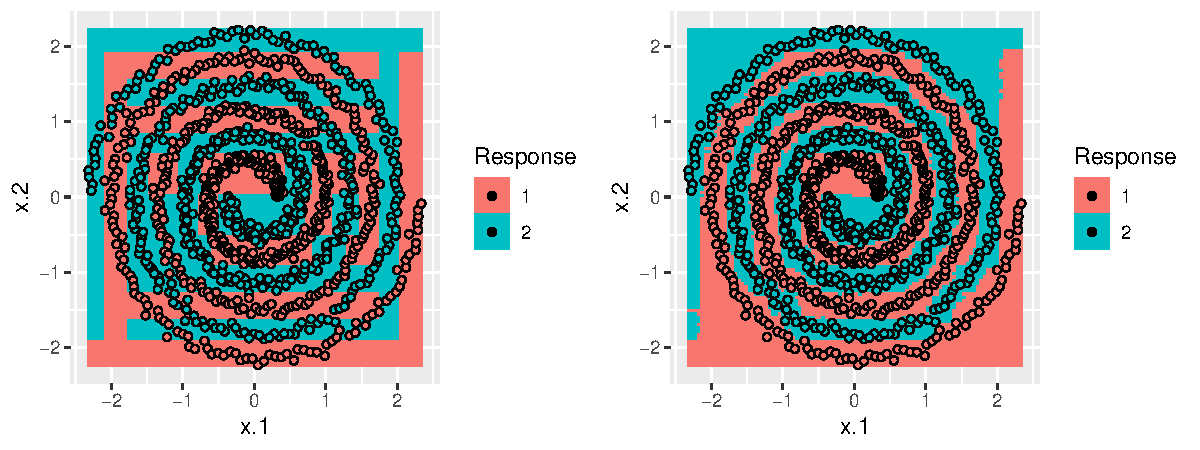
\includegraphics[width=\maxwidth]{figure/unnamed-chunk-11-1} 
\begin{kframe}\begin{alltt}
\hlstd{circle1} \hlkwb{=} \hlstd{mlr3viz}\hlopt{::}\hlkwd{plot_learner_prediction}\hlstd{(rp, task.circle)} \hlopt{+}
  \hlkwd{guides}\hlstd{(}\hlkwc{shape} \hlstd{=} \hlnum{FALSE}\hlstd{)}
\end{alltt}
\begin{verbatim}
## INFO  [17:12:25.340] [mlr3]  Applying learner 'classif.rpart' on task 'circle' (iter 1/1)
\end{verbatim}
\begin{alltt}
\hlstd{circle2} \hlkwb{=} \hlstd{mlr3viz}\hlopt{::}\hlkwd{plot_learner_prediction}\hlstd{(rf, task.circle)} \hlopt{+}
  \hlkwd{guides}\hlstd{(}\hlkwc{shape} \hlstd{=} \hlnum{FALSE}\hlstd{)}
\end{alltt}
\begin{verbatim}
## INFO  [17:12:25.448] [mlr3]  Applying learner 'classif.ranger' on task 'circle' (iter 1/1)
\end{verbatim}
\begin{alltt}
\hlkwd{grid.arrange}\hlstd{(circle1, circle2,} \hlkwc{ncol} \hlstd{=} \hlnum{2}\hlstd{)}
\end{alltt}
\end{kframe}
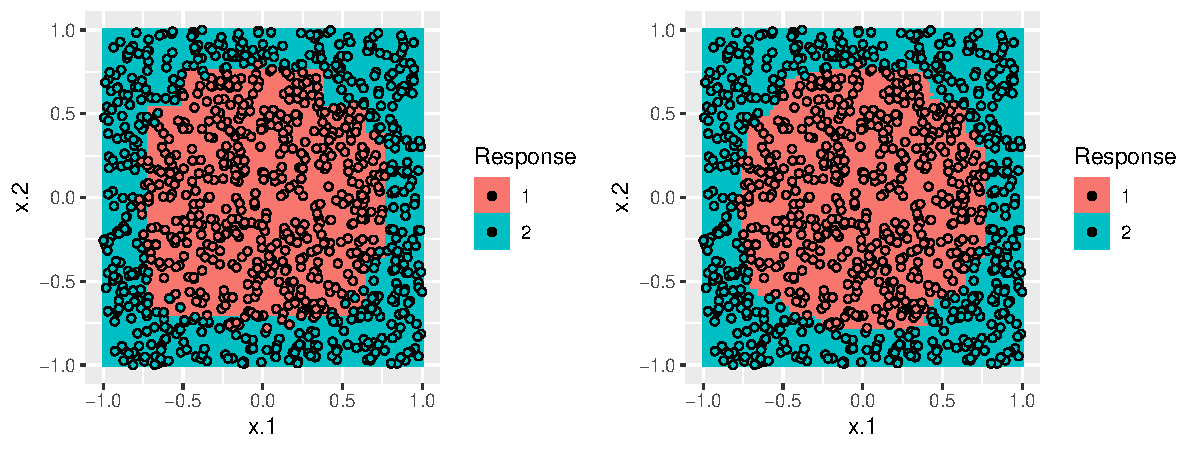
\includegraphics[width=\maxwidth]{figure/unnamed-chunk-11-2} 
\end{knitrout}

}

\dlz
\aufgabe{decision boundaries}{

Generate an artificial dataset with the function call \texttt{mlbench.spirals(n = 500, sd = 0.1)}. (The function \texttt{mlbench.spirals} is part of the \texttt{mlbench} package.) Visualize the decision boundaries of a random forest using the \texttt{classif.ranger} learner from \texttt{mlr3learners}. Create plots with \texttt{plot\_learner\_prediction} from \texttt{mlr3viz} for an increasing number of trees. (Start with \texttt{num.trees = 1}) Explain what you see.
}

\dlz
\loesung{

See
\href{https://github.com/compstat-lmu/lecture_i2ml/blob/master/exercises/forests/ex_rnw/sol_dec_boundaries.R}{R code}
}

\dlz
\aufgabe{random forest implementations}{

Compare two implementations of random forests. One from the package \texttt{randomForest} and one from the package \texttt{ranger}.
Compare them on some datasets (\textbf{hint:} use \texttt{benchmark()}) and measure the test error as well as computation time. Don't use too small datasets or your results will be way to noisy to see meaningful differences.
}

\dlz
\loesung{

See
\href{https://github.com/compstat-lmu/lecture_i2ml/blob/master/exercises/forests/ex_rnw/sol_rf_implementations.R}{R code}
}

\newpage
\aufgabe{spam classification}{

\begin{enumerate}
  \item[a)] Take a look at the \texttt{spam} dataset (\texttt{?mlr3::mlr\_tasks\_spam}).
  Shortly describe what kind of classification problem this is and access the corresponding task predefined in \texttt{mlr3}.

  \item[b)] Use a decision tree to predict spam. Try refitting with different samples. How stable are the trees?

  Hint: Use \texttt{rpart.plot()} from the package \texttt{rpart.plot} to vizualize the trees. (You can access the model of a learner by its class attribute \texttt{model})

  \item[c)] Use the random forest learner \texttt{classif.ranger} to fit the model and state the oob-error.


  \item[d)] Your boss wants to know which variables have the biggest influence on the prediction quality. Explain your approach in words as well as code.

  Hint: use an adequate variable importance filter as described in \url{https://mlr3filters.mlr-org.com/#variable-importance-filters}.
\end{enumerate}
}

\dlz
\loesung{

\begin{enumerate}
  \item[a)]
  The spam data is a binary classification task where the aim is to classify an email as spam or no-spam.

\begin{knitrout}
\definecolor{shadecolor}{rgb}{0.969, 0.969, 0.969}\color{fgcolor}\begin{kframe}
\begin{alltt}
\hlkwd{library}\hlstd{(mlr3)}
\hlkwd{library}\hlstd{(mlr3learners)}
\hlkwd{library}\hlstd{(mlr3filters)}

\hlkwd{tsk}\hlstd{(}\hlstr{"spam"}\hlstd{)}
\end{alltt}
\begin{verbatim}
## <TaskClassif:spam> (4601 x 58)
## * Target: type
## * Properties: twoclass
## * Features (57):
##   - dbl (57): address, addresses, all, business, capitalAve,
##     capitalLong, capitalTotal, charDollar, charExclamation, charHash,
##     charRoundbracket, charSemicolon, charSquarebracket, conference,
##     credit, cs, data, direct, edu, email, font, free, george, hp, hpl,
##     internet, lab, labs, mail, make, meeting, money, num000, num1999,
##     num3d, num415, num650, num85, num857, order, original, our, over,
##     parts, people, pm, project, re, receive, remove, report, table,
##     technology, telnet, will, you, your
\end{verbatim}
\end{kframe}
\end{knitrout}
  \item[b)]

\begin{knitrout}
\definecolor{shadecolor}{rgb}{0.969, 0.969, 0.969}\color{fgcolor}\begin{kframe}
\begin{alltt}
\hlkwd{library}\hlstd{(rpart.plot)}
\end{alltt}


{\ttfamily\noindent\itshape\color{messagecolor}{\#\# Loading required package: rpart}}\begin{alltt}
\hlstd{task_spam} \hlkwb{<-} \hlkwd{tsk}\hlstd{(}\hlstr{"spam"}\hlstd{)}

\hlstd{learner} \hlkwb{<-} \hlkwd{lrn}\hlstd{(}\hlstr{"classif.rpart"}\hlstd{)}
\hlstd{learner}\hlopt{$}\hlkwd{train}\hlstd{(task_spam)}

\hlkwd{rpart.plot}\hlstd{(learner}\hlopt{$}\hlstd{model,} \hlkwc{roundint}\hlstd{=}\hlnum{FALSE}\hlstd{)}
\end{alltt}
\end{kframe}
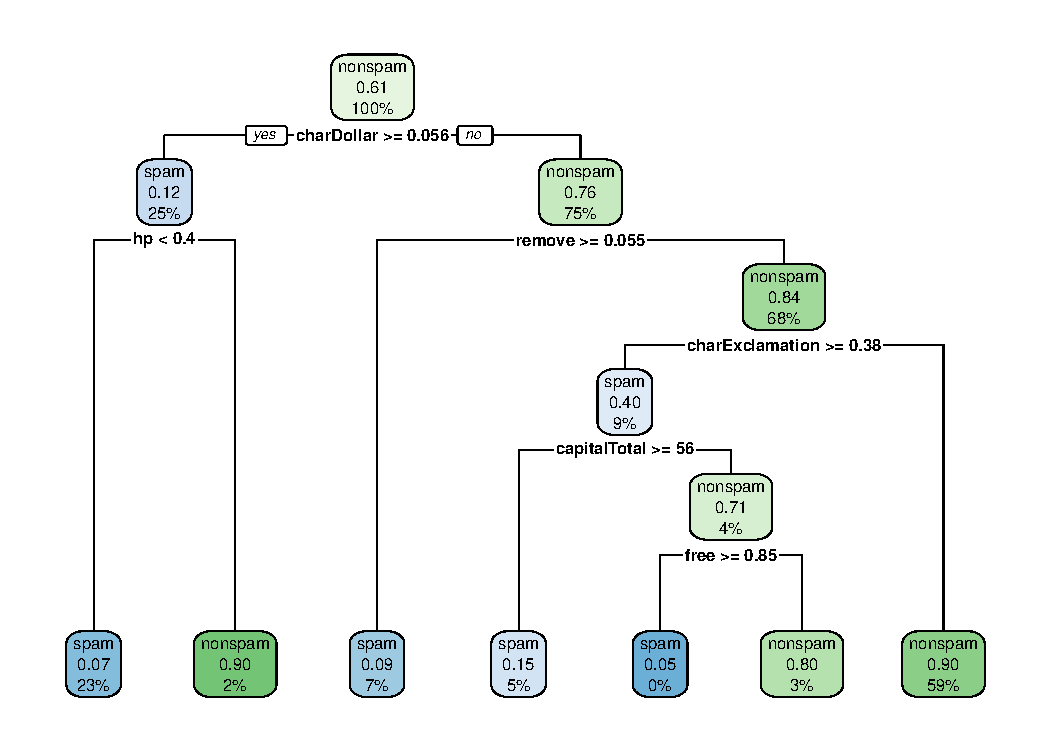
\includegraphics[width=\maxwidth]{figure/unnamed-chunk-13-1} 
\begin{kframe}\begin{alltt}
\hlkwd{set.seed}\hlstd{(}\hlnum{42}\hlstd{)}

\hlstd{subset1} \hlkwb{<-} \hlkwd{sample.int}\hlstd{(task_spam}\hlopt{$}\hlstd{nrow,} \hlkwc{size} \hlstd{=} \hlnum{0.8} \hlopt{*} \hlstd{task_spam}\hlopt{$}\hlstd{nrow)}
\hlstd{subset2} \hlkwb{<-} \hlkwd{sample.int}\hlstd{(task_spam}\hlopt{$}\hlstd{nrow,} \hlkwc{size} \hlstd{=} \hlnum{0.8} \hlopt{*} \hlstd{task_spam}\hlopt{$}\hlstd{nrow)}

\hlstd{learner}\hlopt{$}\hlkwd{train}\hlstd{(task_spam,} \hlkwc{row_ids} \hlstd{= subset1)}
\hlkwd{rpart.plot}\hlstd{(learner}\hlopt{$}\hlstd{model,} \hlkwc{roundint}\hlstd{=}\hlnum{FALSE}\hlstd{)}
\end{alltt}
\end{kframe}
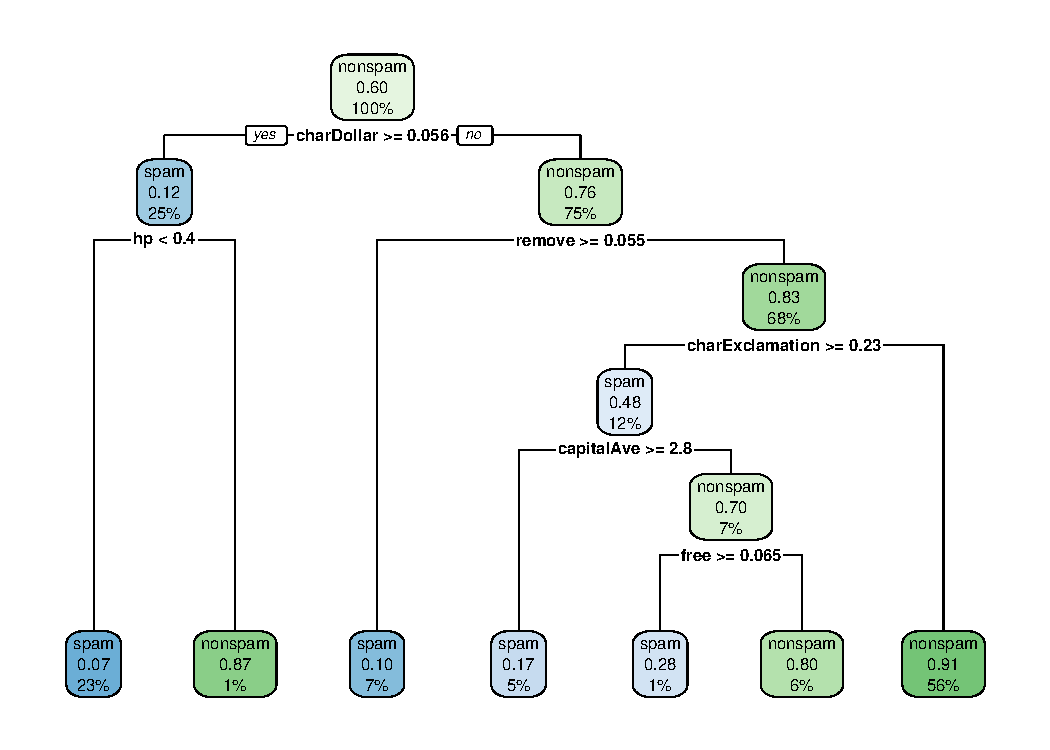
\includegraphics[width=\maxwidth]{figure/unnamed-chunk-13-2} 
\begin{kframe}\begin{alltt}
\hlstd{learner}\hlopt{$}\hlkwd{train}\hlstd{(task_spam,} \hlkwc{row_ids} \hlstd{= subset2)}
\hlkwd{rpart.plot}\hlstd{(learner}\hlopt{$}\hlstd{model,} \hlkwc{roundint}\hlstd{=}\hlnum{FALSE}\hlstd{)}
\end{alltt}
\end{kframe}
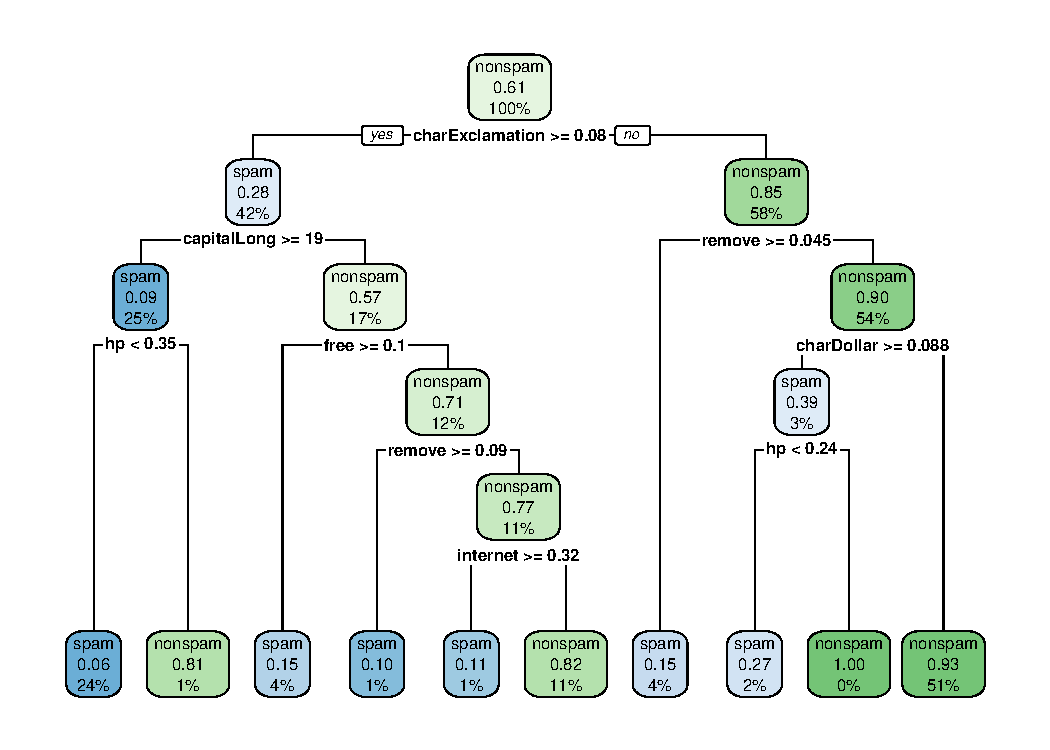
\includegraphics[width=\maxwidth]{figure/unnamed-chunk-13-3} 
\end{knitrout}
  Observation: Trees with different sample find different split points and variables, leading to different trees!

  \item[c)]

\begin{knitrout}
\definecolor{shadecolor}{rgb}{0.969, 0.969, 0.969}\color{fgcolor}\begin{kframe}
\begin{alltt}
\hlstd{learner} \hlkwb{<-} \hlkwd{lrn}\hlstd{(}\hlstr{"classif.ranger"}\hlstd{,} \hlstr{"oob.error"} \hlstd{=} \hlnum{TRUE}\hlstd{)}
\hlstd{learner}\hlopt{$}\hlkwd{train}\hlstd{(}\hlkwd{tsk}\hlstd{(}\hlstr{"spam"}\hlstd{))}

\hlstd{model} \hlkwb{<-} \hlstd{learner}\hlopt{$}\hlstd{model}

\hlstd{model}\hlopt{$}\hlstd{prediction.error}
\end{alltt}
\begin{verbatim}
## [1] 0.04542491
\end{verbatim}
\end{kframe}
\end{knitrout}

  \item[d)]

Variable importance in general measures the contributions of features to a model.
One way of computing the variable importance of the j-th variable is based on permutations of the OOB observations of the j-th variable, which measures the mean deacrease of the predictive accuracy induced by this permutation. To determine the $n$ variables with the biggest influence on the prediction quality, one can choose the $n$ variables with the highest variable importance based on permutations of the OOB,
e.g. for $n=5$:

\begin{knitrout}
\definecolor{shadecolor}{rgb}{0.969, 0.969, 0.969}\color{fgcolor}\begin{kframe}
\begin{alltt}
\hlstd{learner} \hlkwb{<-} \hlkwd{lrn}\hlstd{(}\hlstr{"classif.ranger"}\hlstd{,} \hlkwc{importance} \hlstd{=} \hlstr{"permutation"}\hlstd{,} \hlstr{"oob.error"} \hlstd{=} \hlnum{TRUE}\hlstd{)}
\hlstd{filter} \hlkwb{<-} \hlkwd{flt}\hlstd{(}\hlstr{"importance"}\hlstd{,} \hlkwc{learner} \hlstd{= learner)}
\hlstd{filter}\hlopt{$}\hlkwd{calculate}\hlstd{(}\hlkwd{tsk}\hlstd{(}\hlstr{"spam"}\hlstd{))}
\hlkwd{head}\hlstd{(}\hlkwd{as.data.table}\hlstd{(filter),} \hlnum{5}\hlstd{)}
\end{alltt}
\begin{verbatim}
##            feature      score
## 1:     capitalLong 0.04644338
## 2:              hp 0.04125252
## 3: charExclamation 0.03977957
## 4:          remove 0.03827180
## 5:      capitalAve 0.03424298
\end{verbatim}
\end{kframe}
\end{knitrout}

\end{enumerate}
}

% ------------------------------------------------------------------------------
% PAST EXAMS
% ------------------------------------------------------------------------------

\dlz
\exexams
\lz

\aufgabeexam{WS2020/21}{main}{2}{

The table below shows $\D = \Dset $, a data set with 
$n$ = 5 observations of a continuous target variable $y$ and a continuous, 
1-dimensional feature variable $\xv$. In the following, we aim at predicting 
$y$ with a machine learning model that takes $\xv$ as input.

\begin{tabular}{ | c | c | c |}
\hline
ID  &  $\xv$  &  $y$  \\  \hline
1   &  1.0    &  3.1  \\
2   &  5.2    &  0.5  \\
3   &  2.7    &  1.7  \\
4   &  1.1    &  4.5  \\
5   &  1.5    &  2.7  \\
\hline
\end{tabular}

\begin{enumerate}

  \item We train a random forest with L2 loss $\Lxy = 0.5(y-\fx)^2$ and 
  $\texttt{num.trees} = 3$ trees. The results of the training and all estimated 
  split points and predicted labels can be found in the R script \texttt{rf.R}. 
  To prevent differing numbers due to technical reasons, you see the output of 
  \texttt{ranger::treeInfo()} in the following table. Predict the label $y$ for 
  a new observation $\xv_* = 2$ with the random forest as given in the table 
  below. State the entire manual calculation, i.e., the entire path of the 
  observation through the trees in detail. (You are allowed to use R to 
  cross-check your solution, but we will only grade your manual computations -- 
  for full points, you have to describe your calculations thoroughly.) 
  
  \item Compute the proximities of the 5 training observations, using the random 
  forest. In \texttt{rf.R} you see the skeleton of a function 
  \texttt{get\_prox\_matrix()}. Complete this function and apply it to the 
  predictions of the individual trees of the random forest, which are 
  precomputed in the R script for you and stored in the matrix 
  \texttt{pred\_mat}. Print the results. This is an R question. As a solution, 
  hand in a completed version of \texttt{rf.R}. No hand-written solution is 
  allowed here.
  
  \item Use the proximities matrix given below for outlier detection: Which 
  observations are the most likely candidates for being an outlier and why? 
  State the IDs of the respective observations.
  
\end{enumerate}

}

\dlz

\loesung{

\begin{enumerate}

  \item

\begin{tabular}{r|r|r|r|l|r|l|r}
\hline
nodeID & leftChild & rightChild & splitvarID & splitvarName & splitval & terminal & prediction\\
\hline
0 & 1 & 2 & 0 & x & 1.30 & FALSE & NA\\
\hline
1 & 3 & 4 & 0 & x & 1.05 & FALSE & NA\\
\hline
2 & NA & NA & NA & NA & NA & TRUE & 2.7\\
\hline
3 & NA & NA & NA & NA & NA & TRUE & 3.1\\
\hline
4 & NA & NA & NA & NA & NA & TRUE & 4.5\\
\hline
\end{tabular}


\begin{tabular}{r|r|r|r|l|r|l|r}
\hline
nodeID & leftChild & rightChild & splitvarID & splitvarName & splitval & terminal & prediction\\
\hline
0 & 1 & 2 & 0 & x & 1.30 & FALSE & NA\\
\hline
1 & 3 & 4 & 0 & x & 1.05 & FALSE & NA\\
\hline
2 & 5 & 6 & 0 & x & 2.10 & FALSE & NA\\
\hline
3 & NA & NA & NA & NA & NA & TRUE & 3.1\\
\hline
4 & NA & NA & NA & NA & NA & TRUE & 4.5\\
\hline
5 & NA & NA & NA & NA & NA & TRUE & 2.7\\
\hline
6 & NA & NA & NA & NA & NA & TRUE & 1.7\\
\hline
\end{tabular}


\begin{tabular}{r|r|r|r|l|r|l|r}
\hline
nodeID & leftChild & rightChild & splitvarID & splitvarName & splitval & terminal & prediction\\
\hline
0 & 1 & 2 & 0 & x & 1.30 & FALSE & NA\\
\hline
1 & 3 & 4 & 0 & x & 1.05 & FALSE & NA\\
\hline
2 & NA & NA & NA & NA & NA & TRUE & 2.7\\
\hline
3 & NA & NA & NA & NA & NA & TRUE & 3.1\\
\hline
4 & NA & NA & NA & NA & NA & TRUE & 4.5\\
\hline
\end{tabular}


  \begin{itemize}
    \item Tree 1:
    \begin{itemize}
      \item Split 1: left child since $2<3.15 $
      \item End node: Prediction 4.5
    \end{itemize}
    \item Tree 2:
    \begin{itemize}
      \item Split 1: left child since $2<2.1$
      \item Split 2: right child since $2>1.3$
      \item End node: Prediction 2.7
    \end{itemize}
    \item Tree 3:
    \begin{itemize}
      \item Split 1: right child since $2>1.9$
      \item Split 2: left child since $2<3.95$
      \item End node: Prediction 1.7
    \end{itemize}
    Final prediction is the mean of the 3 values: 2.97
  \end{itemize}

  \item Model solution somewhere in exam folder?

  \item

\begin{tabular}{l|r|r|r|r|r}
\hline
  & 1 & 2 & 3 & 4 & 5\\
\hline
1 & NA & 0.00 & 0.00 & 0 & 0.00\\
\hline
2 & 0 & NA & 1.00 & 0 & 0.67\\
\hline
3 & 0 & 1.00 & NA & 0 & 0.67\\
\hline
4 & 0 & 0.00 & 0.00 & NA & 0.00\\
\hline
5 & 0 & 0.67 & 0.67 & 0 & NA\\
\hline
\end{tabular}



\end{enumerate}
}

% ------------------------------------------------------------------------------

\aufgabeexam{WS2020/21}{retry}{2}{

The table below shows $\D = \Dset $, a data set with 
$n$ = 10 observations of a binary target variable \texttt{PlayTennis} and two 
binary feature variables \texttt{Temperature} and \texttt{Weather}. 
In the following, we aim at predicting \texttt{PlayTennis} with a machine 
learning model that takes \texttt{Temperature} and \texttt{Weather} as input.

\resizebox{0.88\textwidth}{!}{%
\begin{tabular}{|r|cccccccccc|}
  \hline
ID & 1 & 2 & 3 & 4 & 5 & 6 & 7 & 8 & 9 & 10 \\
  \hline
Temperature & cool & cool & cool & hot & hot & cool & hot & cool & cool & hot \\
  Weather & rain & rain & sunny & sunny & sunny & rain & rain & sunny & sunny & sunny \\
  \hline
  PlayTennis & no & no & yes & no & yes & no & yes & yes & yes & yes \\
   \hline
\end{tabular}
}
}

\begin{enumerate}
  \item We train a random forest with $\texttt{num.trees} = 3$ trees. 
  The results of the training and all estimated split points and predicted 
  labels can be found in the R script \texttt{snd\_rf.R}. 
  To prevent differing numbers due to technical reasons, you see the output of 
  \texttt{ranger::treeInfo()} in the following table. 
  Predict the label \texttt{PlayTennis} for a new observation 
  $\xv_* = (cool, rain)^\top$ with the random forest as given in the table 
  below. State the entire manual calculation, i.e., the entire path of the 
  observation through the trees in detail. (You are allowed to use R to 
  cross-check your solution, but we will only grade your manual computations -- 
  for full points, you have to describe your calculations thoroughly.) 
\end{enumerate}

\newpage
\loesung{

\begin{enumerate}
  \item   
  

\begin{tabular}{r|r|r|r|l|r|l|l}
\hline
nodeID & leftChild & rightChild & splitvarID & splitvarName & splitval & terminal & prediction\\
\hline
0 & 1 & 2 & 0 & temperature & 1.5 & FALSE & NA\\
\hline
1 & NA & NA & NA & NA & NA & TRUE & no\\
\hline
2 & NA & NA & NA & NA & NA & TRUE & yes\\
\hline
\end{tabular}


\begin{tabular}{r|r|r|r|l|r|l|l}
\hline
nodeID & leftChild & rightChild & splitvarID & splitvarName & splitval & terminal & prediction\\
\hline
0 & 1 & 2 & 0 & temperature & 1.5 & FALSE & NA\\
\hline
1 & NA & NA & NA & NA & NA & TRUE & yes\\
\hline
2 & NA & NA & NA & NA & NA & TRUE & yes\\
\hline
\end{tabular}


\begin{tabular}{r|r|r|r|l|r|l|l}
\hline
nodeID & leftChild & rightChild & splitvarID & splitvarName & splitval & terminal & prediction\\
\hline
0 & 1 & 2 & 0 & temperature & 1.5 & FALSE & NA\\
\hline
1 & 3 & 4 & 1 & weather & 1.5 & FALSE & NA\\
\hline
2 & 5 & 6 & 1 & weather & 1.5 & FALSE & NA\\
\hline
3 & NA & NA & NA & NA & NA & TRUE & no\\
\hline
4 & NA & NA & NA & NA & NA & TRUE & yes\\
\hline
5 & NA & NA & NA & NA & NA & TRUE & yes\\
\hline
6 & NA & NA & NA & NA & NA & TRUE & yes\\
\hline
\end{tabular}


  In the R code you can see that cool is class 1, hot is class 2, for 
  temperature and that rain is class 1, sun is class 2 for weather.
  \begin{itemize}
    \item Tree 1: 
    \begin{itemize}
      \item nodeID 0: left child since cool $=1<1.5 \Rightarrow$ nodeID = 1
      \item nodeID 1: left child since rain $=1<1.5 \Rightarrow$ nodeID = 3
      \item nodeID 3 = End node: Prediction 'no'
    \end{itemize}
    \item Tree 2: 
    \begin{itemize}
      \item nodeID 0: left child since rain $=1<1.5 \Rightarrow$ nodeID = 1
      \item nodeID 1: left child since cool $=1<1.5 \Rightarrow$ nodeID = 3
      \item nodeID 3 = End node: Prediction 'no'
    \end{itemize}
    \item Tree 3: 
    \begin{itemize}
      \item nodeID 0: left child since cool $=1<1.5 \Rightarrow$ nodeID = 1
      \item nodeID 1 = End node: Prediction 'no'
    \end{itemize}
    Final prediction is the majority vote of the 3 values: 'no'
  \end{itemize}
\end{enumerate} 
}

% ------------------------------------------------------------------------------
% INSPO
% ------------------------------------------------------------------------------

\dlz
\exinspo
\end{document}
